
An aspect requiring some care is the presence of $Z$+jets in the CRHigh from $VH(\rightarrow b\bar{b})$, as displayed in Figure \ref{fig:vhbbDRCR02L}. This $V$+hf (heavy flavour: mostly $bb$) and  is taken directly from $VH(\rightarrow b\bar{b})$ and will have an impact on the similarly named background in $VH(\rightarrow c\bar{c})$, as shown in the pull plots of Figure \ref{fig:Vpulls}

\begin{figure}[h!]
%\hspace{-2.0cm}
\center
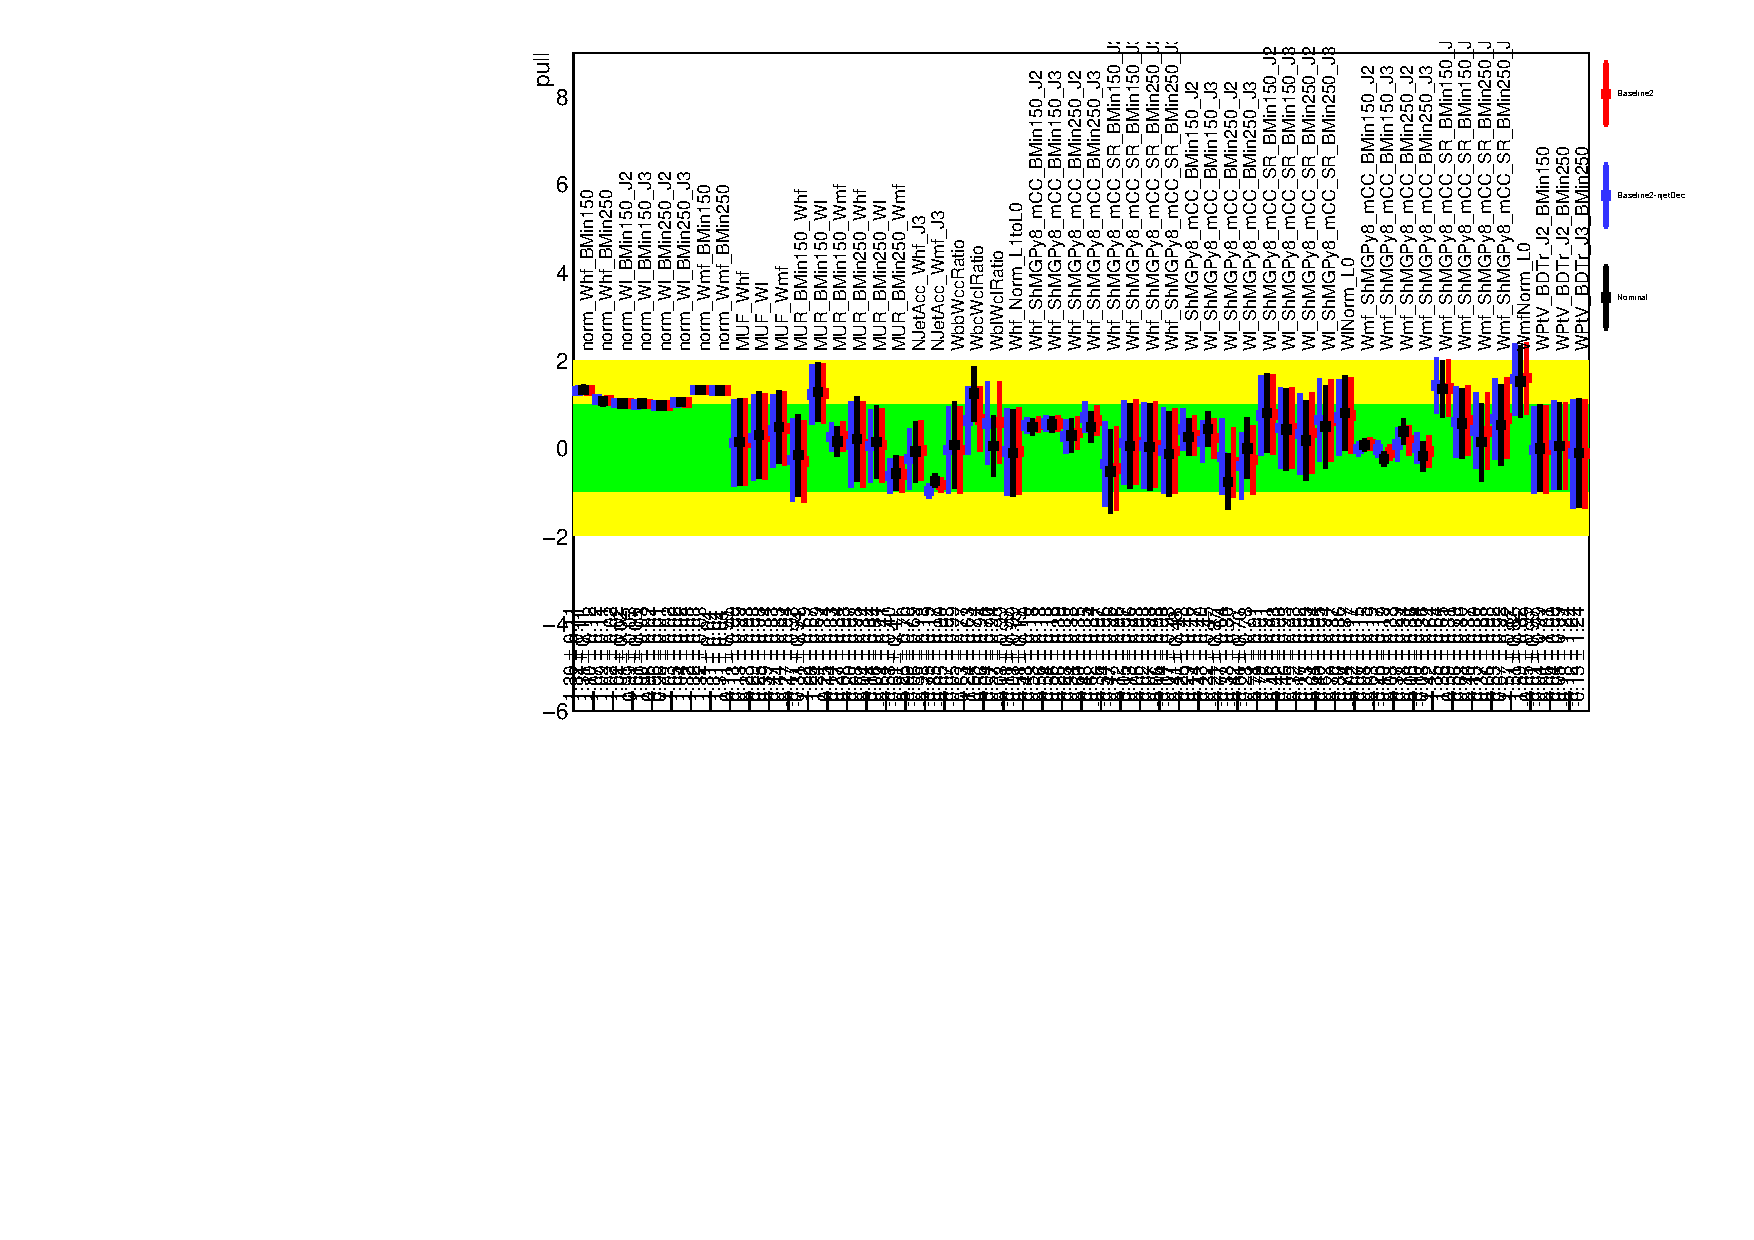
\includegraphics[scale=0.6]{Images/VH/pc3_v10_nomNjet_baseline2_nJetDecorr_012L/NP_Wjets.pdf}
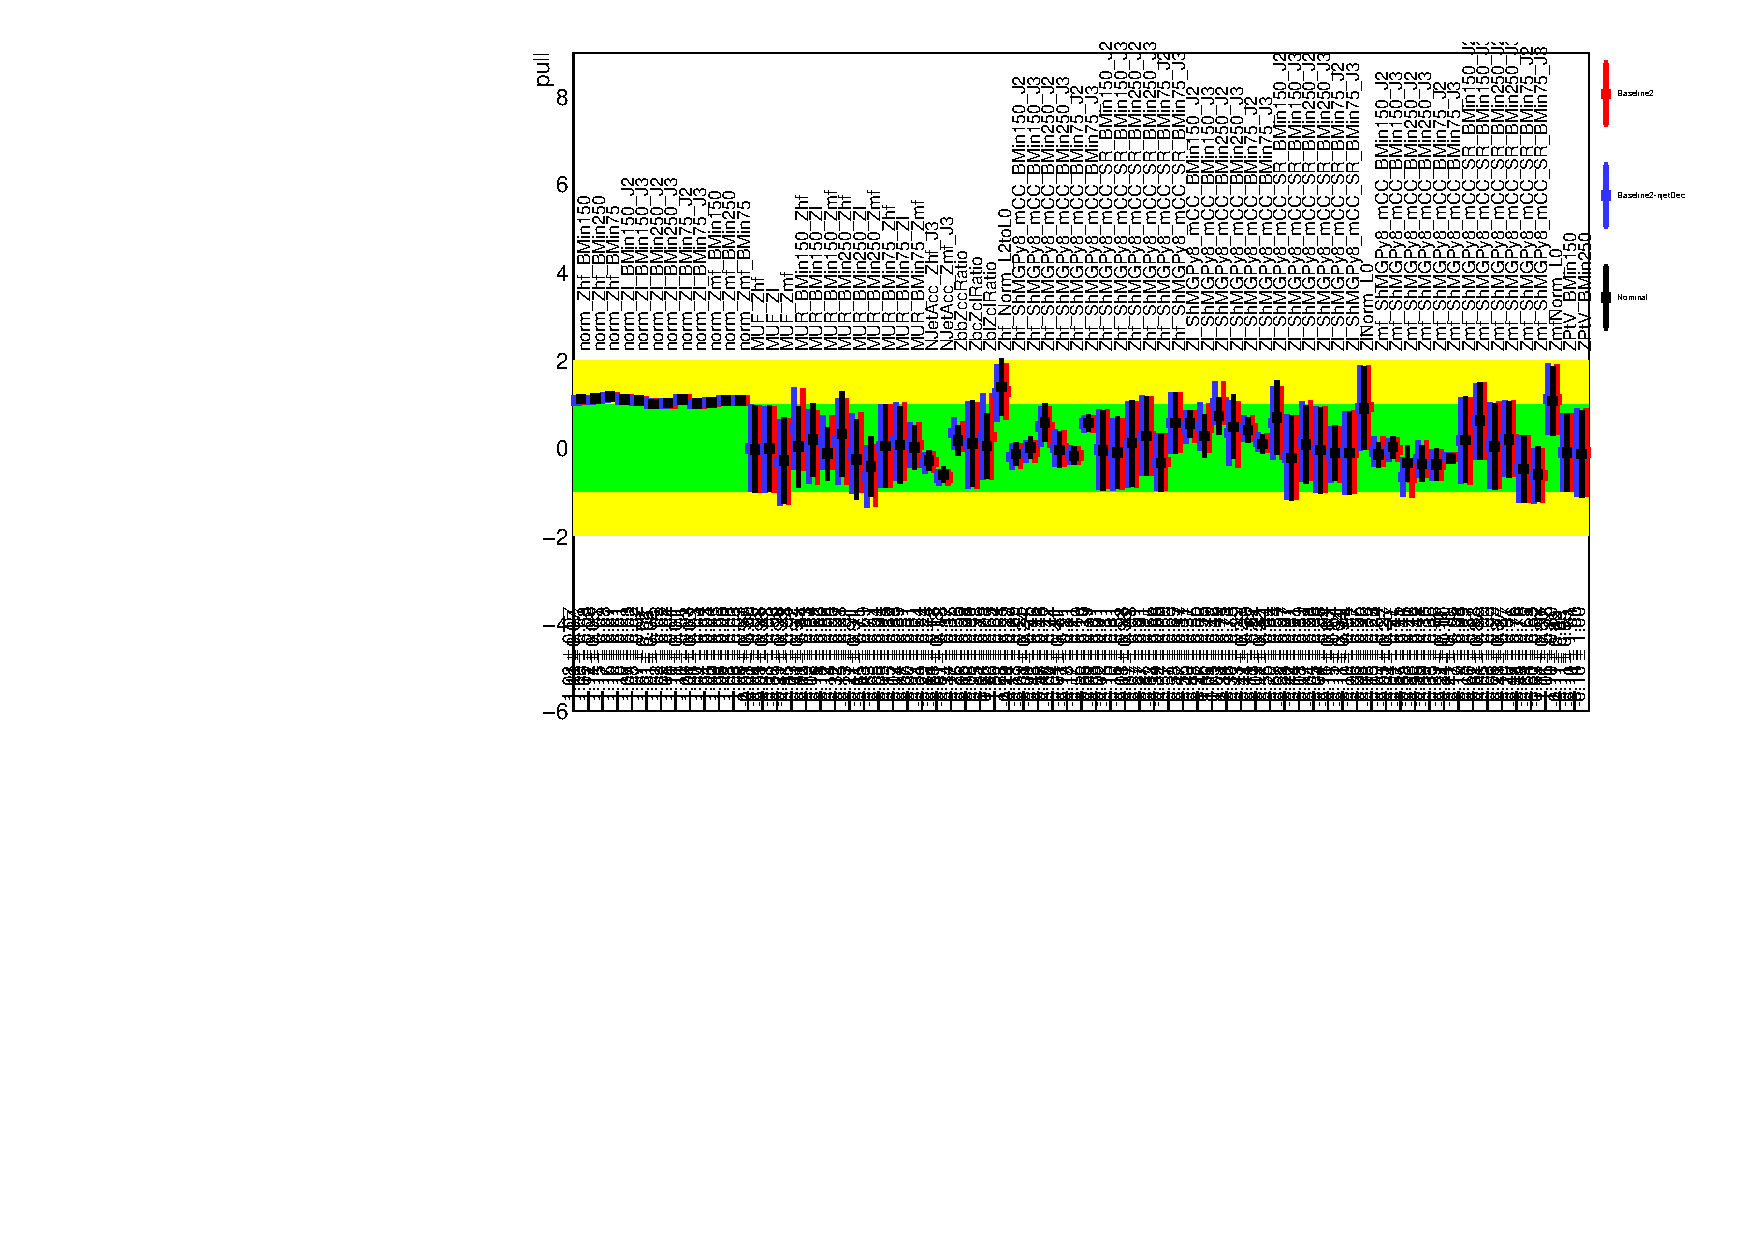
\includegraphics[scale=0.6]{Images/VH/pc3_v10_nomNjet_baseline2_nJetDecorr_012L/NP_Zjets.pdf}\\
\caption{Pull plots for the 012L fit with the several baselines. Top: $W$+jets NPs; $Z$+jets NPs. Black: nominal; red: baseline 2; blue: baseline 2 + nJetDec.} 
\label{fig:Vpulls}
\end{figure}

